\documentclass{mprop}
\usepackage{graphicx}

% alternative font if you prefer \usepackage{times}

% for alternative page numbering use the following package and see documentation
% for commands \usepackage{fancyheadings}


% other potentially useful packages \uspackage{amssymb,amsmath}
\usepackage{url}
%\usepackage{fancyvrb} \usepackage[final]{pdfpages}

\begin{document}

%%%%%%%%%%%%%%%%%%%%%%%%%%%%%%%%%%%%%%%%%%%%%%%%%%%%%%%%%%%%%%%%%%%
\title{Is Technical Debt Real?}
\author{Ovidiu Popoviciu}
\date{18th December 2017}
\maketitle
%%%%%%%%%%%%%%%%%%%%%%%%%%%%%%%%%%%%%%%%%%%%%%%%%%%%%%%%%%%%%%%%%%%

%%%%%%%%%%%%%%%%%%%%%%%%%%%%%%%%%%%%%%%%%%%%%%%%%%%%%%%%%%%%%%%%%%%
\tableofcontents 
\newpage
%%%%%%%%%%%%%%%%%%%%%%%%%%%%%%%%%%%%%%%%%%%%%%%%%%%%%%%%%%%%%%%%%%%

%%%%%%%%%%%%%%%%%%%%%%%%%%%%%%%%%%%%%%%%%%%%%%%%%%%%%%%%%%%%%%%%%%%
\section{Introduction}
\label{intro}

The phenomenon of technical debt has matured in recent years with numerous
scientific experiments conducted for its identification, measurement and
management. Initially coined in 1993 \cite{Cunningham1993}, it defined the
concept of not quite right code that provided gains in the short term. Thus
technical debt might be useful in achieving immediate deadlines with possible
software quality sacrifices that might be negative for future work. Negative
consequences in the long term could see software complexity growth, the
prevalence of bugs and defects, decreased team productivity and augmented work
effort, leading to increased costs of development, infrastructure and
management. The phenomenon affects daily work of developers, project managers
and stakeholders of the business. 

The definition of technical debt has been updated since then, spanning not just
activities related to code implementation but the entire software development
environment. The scientific community identified multiple types of debts
\cite{Li2015}, each with its advantages and consequences if not handled
accordingly. Although industry practitioners are aware of its presence
\cite{Codabux2013} \cite{Lim2012}, there is no standard way of measuring the
current and future impact of technical debt on development and costs of the
team. Additionally, due to lack of vocabulary and complexities of the
phenomenon, developers find it difficult to convey their concerns to project
stakeholders \cite{Kruchten2012}.

The primary research objective is to analyse work effort of feature
implementations within software projects with the purpose of identifying extra
work in the context of technical debt. An additional objective is to understand
how the measure of technical debt varies with software evolution and what types
of features incur or reduce its presence. The research questions have been
organised using the Goal-Question-Metric approach \cite{VanSolingen2002}:
\begin{itemize}
	\item \textbf{RQ1}. Can technical debt be measured in the context of work
	effort?
	      \begin{itemize}
		      \item \textbf{RQ1.1}: What was the difference (delta) in the
		            estimated work effort for a feature and the practical work
		            effort?
			  \item \textbf{RQ1.2}: What was the level of technical debt across
		            feature changesets at the time of implementation?
		      \item \textbf{RQ1.3}: How does the work effort delta vary with the
		            magnitude of technical debt?
		  \end{itemize}
	\item \textbf{RQ2}: What are the development patterns surrounding feature
	      lifecycle?
	      \begin{itemize}
		      \item \textbf{RQ2.1}: At what checkpoints in feature development
		            is technical debt reduction (refactoring) most prominent?
		      \item \textbf{RQ2.2}: What type of work items incur the most
					technical debt?
	      \end{itemize}
\end{itemize}

The main questions RQ1 and RQ2 will be tackled by answering their following
subquestions. The following metrics will be computed and analysed:
\begin{itemize}
	\item The \textbf{practical work effort} spent on feature implementation
	will be calculated by leveraging data from the team's issue tracker and
	version control repository.
	\item The level of \textbf{technical debt} in the system at the time of
	implementation will be measured in terms of code smells and bad coding
	practices.
	\item The \textbf{extra effort} spent on feature implementation will be
	derived as the difference between the estimated and practical effort
	measurements. 
\end{itemize}

The study will use both open-source and commercial projects in order understand
the contrast between the two worlds in the context of technical debt work
effort. We will select data candidates according to various criteria items such
as development model, version control system, availability of initially
estimated work effort data and suitability of code quality tools.

If successful, the study will increase awareness of technical debt in all areas
of the software development environment. Developers will know which code smells
and bad practices have the most impact on their productivity. Project managers
will recognise the costs of debt items within the system and assign appropriate
refactoring activities for each development iteration. Stakeholders will grasp
the impact of incurring technical debt and the effects on the costs of present
and future development of new features. Additionally, the study will highlight
refactoring development patterns of feature development lifecycle. To the best
of my knowledge, this is the first study to highlight technical debt interest
from the perspective of work effort and drill down into the development patterns
of technical debt accrual by increasing the granularity of data.

The proposal is structured as follows. Section \ref{lit-review} highlights
related work on technical debt by covering definition, types, identification,
measurement and management within software teams. Section \ref{proposed-work}
underlines future steps of the study while section \ref{work-plan} outlines
deadlines and deliverables of this experiment.

%%%%%%%%%%%%%%%%%%%%%%%%%%%%%%%%%%%%%%%%%%%%%%%%%%%%%%%%%%%%%%%%%%%
\section{Background Survey}
\label{lit-review}

\subsection{Study Design}

Technical debt has become a broad topic in the scientific community over the
past few years. Many studies highlight the identification, measurement and
management of debt, each applied on a specific or multiple domains, each with
its advantages and disadvantages, each with many contributions and limitations.

The following topics have been explored for conducting a thorough literature
survey:
\begin{itemize}
	\item definitions of technical debt;
	\item types of debt;
	\item identification;
	\item measurement of principal and interest;
	\item code quality tools;
	\item management of debt;
	\item industry case studies.
\end{itemize}

First of all, we wanted to understand how the scientific community defined the
metaphor, its limitations, applications and consequences. Since the term
\emph{debt} comes from a financial terminology, it was ideal to understand the
metaphor in more detail. Second of all, it was essential to understand the types
of technical debt discussed in the community along with ideas from industry
practitioners. Practitioners provide valuable information as they deal with
technical debt and its possible costs on a daily basis. Third of all,
identification of technical debt and code quality tools was vital as they
provide a way to highlight code violations in the system's source code. This
step was necessary since this study will use code quality tools to highlight
possible code smells and assess their impact. Fourth of all, measurement and
calculation of technical debt was an important topic since it is difficult to
aggregate such a complex phenomenon into a single value. Lastly, of extreme
value to proprietary projects is the management of technical debt. This topic
included finding studies on managing debt within Agile methodologies and
practices that help guard against it.

The primary source of information was the Workshop on Managing Technical Debt,
with many papers of its yearly workshop included in this study. The data sources
were ACM Digital Library and IEEE Xplore Digital Library, found through
searching terms on Google Scholar. Additional techniques for finding new papers
included the snowballing technique which pointed to relevant studies in the
domain of software refactoring. Although the study includes approximately 40
papers, it does not include all papers related to technical debt. The literature
search focused mainly on code and design debt, as well as tools and management
practices to combat these two types of debt.

\subsection{Definition, Perspectives and Types}
\label{section:def}

% Ward Cunningham - WyCash Portfolio Management System
Technical debt is a metaphor termed by Cunningham, in his note on the WyCash
Portfolio Management System \cite{Cunningham1993}. In the report, Cunningham
mentioned that ``\textit{shipping first time code is like going into debt}'' and
that as the system evolves new features would become more and more difficult to
implement. This phenomenon was due to feature-rich projects being shipped to
customers early but poorly written with little or no consideration to quality
and future work.

\begin{figure}
	\centering
	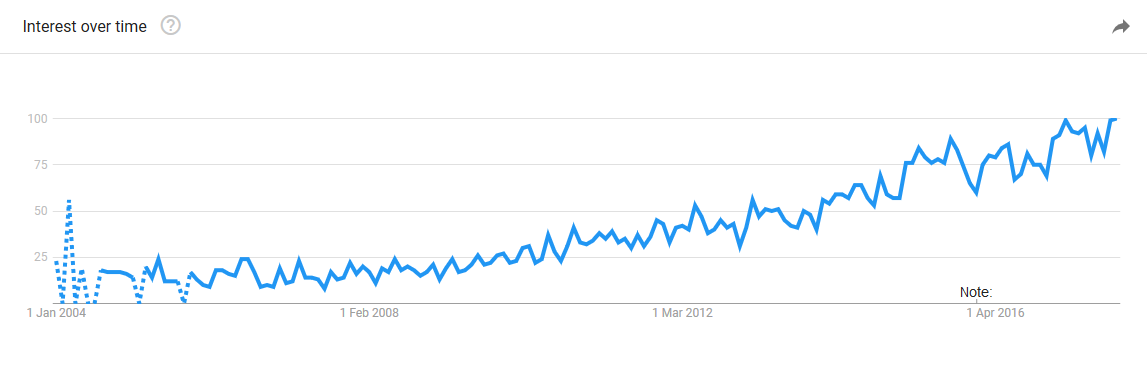
\includegraphics[width=\linewidth]{visualisations/TD_trend.png}
	\caption{Technical Debt Trend from 2004 to Present}
	\label{fig:td-trend}
\end{figure}

% MTD 2010
The metaphor was ignored for a long time, until the late 2000s, when more and
more studies started to explore the phenomenon and possible management
techniques. A figure of the popularity of Technical Debt from 2004 to present
can be seen in Figure \ref{fig:td-trend}, information provided by Google Trends
\cite{GoogleTrends}. The \textit{y} axis represents the interest in technical
debt over time (\textit{x} axis). A value of 100 represents peak search interest
popularity. The term was not as popular during the first years of the century
moreover, gained traction from 2010, as more and more studies became widely
available.

Thus, the first workshop on managing technical debt took place in 2010, where an
initial research agenda was proposed for the future of software engineering
field. Since then, workshops have been held every year, which consisted
seminars, presentations and brainstorming sessions on aspects such as:
definition \cite{Kruchten2012} \cite{Theodoropoulos2011} \cite{Schmid2013},
identification \cite{Ernst2012}, measurement \cite{Letouzey2012}
\cite{Curtis2012} \cite{Nugroho2011} \cite{Zazworka2011} \cite{Fontana2012}
\cite{Bohnet2011}, management \cite{Guo2011} \cite{Zazworka2011Prioritise}
\cite{Seaman2012} and industry case studies \cite{Lim2012}
\cite{Morgenthaler2012} \cite{Codabux2013} \cite{Holvitie2014}
\cite{Klinger2011}.

% from metaphor to theory and practice
The definition of technical debt relies heavily on the perspective of the viewer
and her responsibility within the software development environment. Developers
view technical debt as a list of software quality issues and correlate it with
lack of time to implement features "\textit{properly}" \cite{Codabux2013}.
Product managers and stakeholders view it as a strategy, a way to defer quality,
well-designed work for quick wins to satisfy particular business requirements,
such as Time to Market (TTM). These two perspectives are widely different, with
developers prioritising ``invisible'' code perfection while management is
focusing on the rapid development of ``visible'', selling point features.
Kruchten et al. \cite{Kruchten2012} defined technical debt as technological gaps
between development teams and management where a gap is the evolution of
context, specific to a decision taken in the past. These gaps could be decisions
that seemed correct when approved. However with the passing of time, it
unintentionally incurred debt. For example, no tool would have predicted what
frameworks and languages would have existed in the future or how requirements
would have changed to prepare accordingly. As a consequence, the authors stated
that technical debt is not the collection of code quality violations within the
results of static code analysers but, a phenomenon which is heavily reliant on
the present and future evolution.


% from a stakeholder's perspective
However, most strategic decisions on the future evolution of the project come
from management. Unfortunately, stakeholders might not know the metaphor of
technical debt, its current measurement and whether it impacts costs of
development. Their fundamental focus consists of increasing business value
through the addition of visual features, rather than looking for investment in
the quality of the software produced \cite{Lim2012}. As a result, new features
are prioritised and pressured on being delivered as early and as quickly as
possible. These types of issues affect the \textbf{extrinsic quality} of
software and are "visible". For example, an external quality characteristic is
usability. Deferring user experience work while ignoring user interface bugs
might force users of the system to find "ways around" certain tasks. The result
negatively impacts user productivity and the general usefulness of the product.
Extrinsic characteristics are important to the business because they are ``sell
points'' of the product. On the other hand, \textbf{intrinsic quality}
characteristics of software are the low-level issues such as code smells,
best-practices violations that might slow down development of new features
unless refactoring processes are applied. Theodoropoulos et al.
\cite{Theodoropoulos2011} considered that intrinsic and extrinsic software
quality characteristics are interdependent and deferring quality maintenance in
one area may affect other areas of quality. For example, improper data
validation in the business logic layer of the system may impact downstream
components, such as user interface, and produce bugs within the system.


% on the limits of td metaphor TODO: define principal and interest
Although the use of finance terms may simplify technical characteristics of
software quality in the dialogue between development teams and stakeholders, the
analogy breaks down as studied by Schmid et al. \cite{Schmid2013}. In their
study, the authors had identified shortcomings in the financial metaphor
established by Ward Cunningham \cite{Cunningham1993} and found points where it
breaks down. In the financial domain, debt is a well-known arrangement between
two parties where one party borrows a fixed amount of money from the other party
\cite{debt-investopedia}. The most common types of debt are loans, where the
terms of the arrangement dictate that the amount of money borrowed must be paid
back in full after a fixed period, along with fixed interest payments paid
annually.

Schmid et al. \cite{Schmid2013} identified three major points where the analogy
breaks down:
\begin{itemize}
	\item \textit{Unit of measurement}. In finance, there is a precise unit of
	      monetary measurement through the use of international currencies. In
	      contrast, technical debt does not have a standard unit of measurement
	      defined. There are many tools \cite{Fontana2016} that provide a
	      single, quantified and aggregated measure of the amount of time to
	      resolve a software quality issue. Additionally, very few of these
	      tools quantify the consequences of neglecting refactoring activities.
	      The issue of measurement puts a dent in the shared vocabulary between
	      development and stakeholders as mentioned by many practitioners
	      \cite{Lim2012} \cite{Codabux2013}.
	\item \textit{Fixed time period}. Financial debt arrangements have a fixed
	      \textit{maturity date}, the date when the debt must be paid back.
	      Software quality issues do not have a deadline and may be left in the
	      product. Fixing issues through refactoring activities is associated to
	      paying back the debt. However, quality issues may also never have to
	      be paid back if they do not impact productivity.
	\item \textit{Fixed interest}. A loan arrangement additionally consists of
	      fixed interest payments measured as a percentage of the loan value,
	      paid on an annual or bi-annual basis. The interest compensates for the
	      risk taken by the lender and encourages the loanee to pay back as
	      quickly as possible to avoid paying back too much interest. In
	      reality, there is no such thing as fixed interest dependant on a
	      single factor in technical debt. Interest is difficult to quantify as
	      a matter of principal, and the amount of interest paid after a period
	      depends on future work.
\end{itemize}
Under these circumstances, what is considered "good structure" or "clean code"
is also heavily influenced by future development since future decisions
influence cost impact. As a consequence, no system is \textit{debt free} and
thus fixing every code violation would be an act of gold plating
\cite{Kruchten2012}. Additionally, what is the value of paying back this debt if
the product is competitive and the customers are happy \cite{Lim2012}?

% martin fowler - td quadrants
Fowler \cite{TDMartin} described this type of future debt as
\textbf{inadverted-prudent} debt. A project that was "clean" may find that after
a time that the initial approach taken might not have been the best. He
considered that developers learn on the job to perfect their craft as time
passes. The four quadrants refer to the types of technical debt that one might
encounter in a software project given the approach taken by the development
team. It was one of the four quadrants he defined, as shown in Figure
\ref{fig:td-quandrants}.

\begin{figure}
	\centering
	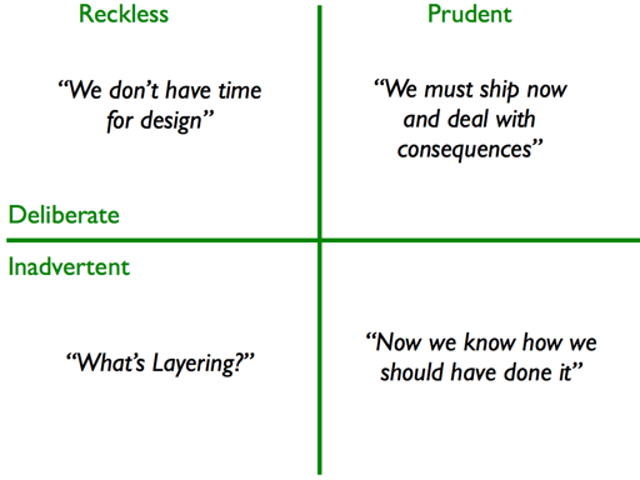
\includegraphics[width=0.5\linewidth]{visualisations/TD_quadrants.png}
	\caption{Martin Fowler's Technical Debt Quadrants}
	\label{fig:td-quandrants}
\end{figure}


% unhedged call option
An alternative metaphor of technical debt \cite{UnhedgedCallOption}, described
bad code similarly using finance terms, but through a different financial
instrument called a call option. ``\textit{An option is a financial derivative
that represents a contract sold by one party (the option writer) to another
party (the option holder). The contract offers the buyer the right, but not the
obligation, to buy (call) or sell (put) a security or other financial asset at
an agreed-upon price (the strike price) during a certain period of time or on a
specific date (exercise date).}'' \cite{option-investopedia}. A call option
gives the right to buy while a put option gives the option holder the right to
sell. In software engineering, if a feature is hacked up quickly and never
touched again, then the project has reaped the rewards. The option ``was not
called''. However, if a new feature were required that would be influenced by
the ``quick and dirty'' work implemented earlier, then the requirement would be
more expensive to fulfil. In this case, the option "was called", though it is
unclear if the development work incurred interest.


% conclusion
Defining software quality issues as a financial metaphor helps bridge vocabulary
shortcomings between developers and stakeholders. It helps management understand
current software development risks and encourages ways of managing these risks.
As Cunningham \cite{Cunningham1993} noted, technical debt may be used as a
strategy to meet business expectations. However, if not repaid promptly, it
``\textit{could bring entire corporations to a standstill}''.

% types of TD
Initially, technical debt solely focused on the internal quality issues of
systems. Such issues could be code smells, code violations, duplicate or
complicated code. However, multiple types of debt have been discovered, spanning
the entire software development environment.


A mapping study, conducted by Li et al. \cite{Li2015}, have analysed 94 studies,
overall dating 1992-2013, and have found ten types of technical debt:
requirements, architecture, design, code, test, build, documentation,
infrastructure, versioning and defect debt. The most prominent type was code
debt, followed by test, architectural, design and documentation.

% architecture debt is the worst - industrial case study
However, in an industrial case study \cite{Codabux2013}, developers considered
that architectural debt is the most difficult to address, due to complexity and
change impact on project modules. Major architectural decisions are not taken in
a vacuum and thus requires group meetings with other developers, software
architects and product managers. The time to reach a consensus on how to
approach architectural changes improve the cost of managing debt.

% technical debt is "technical"
A few of the authors have considered that the metaphor of technical debt only
applies to the low-level, internal quality characteristics such as code, design,
test, architecture rather than gaps within business processes, such as
inadequate quality assurance \cite{Theodoropoulos2011} \cite{Nugroho2011}. Thus
the word ``technical'' in the metaphor. However, business process gaps may
negatively affect projects and incur technical debt as a result.

%%%%%%%%%%%%%%%%%%%%%%%%%%%%%%%%%%%%%%%%%%%%%%%%%%%%%%%%%%%%%%%%%%%
\subsection{Identification and Measurement}

% What are the causes of code TD?

Technical debt may impede future development and delivery of new features if not
managed appropriately \cite{Cunningham1993}. Many authors validated Cunningham's
statement by looking at the most "notorious" code smells \cite{Fowler1999} and
their impact on software projects.

Olbrich et al. \cite{Olbrich2009} studied the impact of two code smells, God
class and Shotgun Surgery, on change-proneness of class entities and size of
changes within two open source systems, Apache Lucene and Apache Xerces. They
gathered data on the number of smells in the systems over revisions and the
distribution of changes on classes suffering from these two smells. The authors
concluded that the number of code smells increases linearly with the evolution
of a system and that classes suffering from the God class smell are 4 to 5 times
more change prone than other non-smelly classes. However, this might be due to a
large amount of functionality within the class suffering from the smell.
Additionally, the study was conducted only on open-source systems and the
results might not apply to commercial software. Additionally, due to limitations
of the tool used to identify code violations, only public Java classes have been
analysed.

In a similar study, Fontana et al. \cite{Fontana2012} studied the impact of
removing code smells on code quality metrics. The authors looked at three
familiar smells: Data class, God class and Duplicated Code. Additional goals
were to find out which code smell incurred the most debt and whether their
impact was related to the domain of product. The metrics impacted were cohesion,
coupling and complexity. They applied refactoring practices for each smell and
the quality metrics were re-evaluated to assess their impact. The results showed
that refactoring of one code smell might provide benefits for some metric
qualities but may negatively impact others. Interestingly, they had found that
the Data Class smell and God class smells might be domain-dependent. For
example, it might be common for the God class smell to appear in algorithm-heavy
systems, such as computer vision applications, while the data class smell may be
more predominant in web applications that hold state.

An exploratory study by Khomh et al. \cite{Khomh2009} empirically analysed the
impact of 29 code smells on the changesets of 9 releases of two open source
systems. They had confirmed the results of the previous studies that code smells
increase the number of changes that software undergoes during its evolution.
Additionally, they had found that classes containing more than one code smell
are more change prone than other classes. Moreover, they found a possible cycle
of repairing smells and better to have new ones between releases.

An interesting idea from all authors \cite{Olbrich2009}, \cite{Fontana2012} and
\cite{Khomh2009} stated that not all code smells have the same consequences on
the code base. A code smell may have been deliberately introduced due to the
nature of project domain. For example, in the case of a system that uses
computer vision algorithm and techniques might be prone to an increased
cyclomatic complexity and God class smells.

% prioritisation by severity - interest probability
Thus, Charalampidou et al. \cite{Charalampidou2017} introduced a study that
assessed the interest probability of code smells, which is the probability of a
code smell to introduce extra changes in future development. Interest
probability was calculated by counting the frequency of each code smell and how
it correlated with the change-proneness of the module where it resides. The
smells studied were Long Method, Conditional Complexity and Duplicated Code. The
results showed that code duplication had the highest interest probability due to
the number of changes required to maintain future development. Additionally,
high cyclomatic method complexity increased amount of changes.

% prioritisation on context
Additionally, prioritising code smells with the highest severity might not be
suitable if the context in which the smell resides will not be referenced in the
future. Therefore, Sae-Lim et al. \cite{Sae-Lim2016} looked at prioritising code
smells according to development context to support a \textit{prefactoring}
stage, where developers clean up code before the implementations of new
features. The authors calculated a value for each code smell, called the
\textit{Context Relevance Index}, based on a list of issues from the project's
issue tracker and the change descriptors of commits in the project version
control. The results of their preliminary study returned a list of ranked code
smells to be resolved as a pre-refactoring step to implementation.

% conclusion of measurement 
Code smells are technical debt items that will increase future development
effort and maintainance costs \cite{Fowler1999}. Industry case studies have
shown that TD items are more likely to be addressed if made visible by
developers within the project's issue tracker \cite{Lim2012}. However, from the
perspective of a project manager, it is essential to understand how much effort
the team puts into technical debt reduction activities and if there is an
associated business value. Hence, after the identification stage, there must
exist a measurement stage of the amount of work effort technical debt will
introduce and the consequences on productivity over time if the team ignores
this debt.

% How to quantify code smell impact?

% introduction
Identification and prioritisation are two of the most critical stages when
dealing with technical debt. Making technical debt items visible was recommended
by many industry practitioners \cite{Lim2012} \cite{Codabux2013}. However, some
have struggled to find a way to measure technical debt and its cumulative effect
over time. This is a particularly important aspect of project managers
responsibility when planning new work for the team. While developers are tasked
with development of new features, managers are responsible for balancing
feature, bug-fixing, infrastructure and refactoring work.

Specifically, a technical debt item raises two important questions:
\begin{itemize}
	\item How much effort does it take to repair now? (\textbf{principal})
	\item What are the future consequences if the team ignores it? (\textbf{interest})
\end{itemize}

Answering these two questions through a quantified measure is the key to a
proactive management of technical debt. The measure depicting the cost of paying
back the debt at the present is called the \textit{principal} while the extra
cost of development when keeping hold of items is called \textit{interest}.
Unfortunately, there is no standardised method, due to difficulties managing
complexities of quantifying work effort and development costs. However, many
have surfaced over the years that define methods for calculating principal and
interest of technical debt items.

Bohnet et al. \cite{Bohnet2011} proposed a tool to bridge the gap between
development teams and corporate managers, by exposing internal system quality
through the use of \textit{software maps}. A software map is a hierarchical
2D/3D view of software artefacts, each represented visually through properties
such as colour, texture and size. The visual properties are associated with a
property of software quality: cyclomatic complexity, lines of code and nesting
levels. Such a visualisation provides both developers and managers with points
of fragility where possible bugs may arise and highlight areas of work to
address. However, the visualisation is technical and might be difficult to
convey results to non-technical stakeholders. Additionally, there is no way to
calculate the principal and interest of the quality issues.

% sqale method for measuring technical debt
Letouzey et al. \cite{Letouzey2012} proposed a different method, called the SQALE
method. The goal was to create a standardised, language-agnostic framework for
assessing the quality of source code by deriving measures for code
characteristics and calculating an overall measure of technical debt. The
framework proposed consisted of four concepts:
\begin{itemize}
	\item Quality Model - defines internal properties of code through a
	      structured three-layer hierarchy (characteristic, sub-characteristic
	      and requirement). For example, a characteristic is maintainability,
	      sub-characteristic is readability, and the requirement is lack of
	      commented code. The hierarchy is defined such that all requirements
	      could be converted into actionable steps. Each requirement defines a
	      remediation index (cost to repair code violations) defined in time,
	      work or capital units.
	\item Analysis Model - measurement of the distance between the current state
	      of the application and the quality target.
	\item Indices - these are the values that represent the costs of paying
	      back debt.
	\item Indicators - provide a visual representation of technical debt indices
	      through ratings.
\end{itemize}
The indices were calculated by summing up the principal of each code violation
and aggregating up into the sub-characteristics and further to the
characteristics of the Quality Model. The technical debt index is provided
through the aggregation of all the characteristics in the Quality Model.
Although the framework provides a useful measurement of technical debt from the
principal of code violations, there is no calculation of interest if TD items
are not reduced and, additionally, it does not take into consideration
architectural debt issues. SonarQube, a continuous code quality tool,
implemented the SQALE method into this product.

Curtis et al. \cite{Curtis2012} summarised the results of a language agnostic
study on a vast database (365M lines of code) of software projects across ten
industries which provided a formula for estimating the principal of TD items.
The authors used CAST's Application Intelligence platform to statically analyse
source code, using 1200 rules of coding best practices. They identified code
violations by analysing source code and aggregated the results into quality
characteristics, or \textit{health factors}. Scores from each health factor were
normalised to a scale of 1 (high risk) to 4 (low risk). The total principal was
estimated by a formula with three parameters: the number of problems, the time
required for each fix and the cost of fixing the issue. Unfortunately, the
methodology did not support the calculation of technical debt interest. The
authors concluded that estimating the interest incurred by a code smell was
difficult since multiple hidden factors influence the results.


Nugroho et al. \cite{Nugroho2011} looked at defining an empirical formula for
quantifying principal and interest. The authors had completed an empirical
analysis of 44 projects within the Software Improvement Group (SIG) using TUViT
software quality assessment method for collecting relevant metrics: lines of
code and duplications. The defined technical debt from an opposite perspective,
as the changes needed to bring a system from its current quality state to the
"ideal" quality. They considered technical debt reduction activities to be
equivalent to a measurement of repair effort (RE). Calculation of this measure
required the number of lines of code that must be changed, the estimated work
effort of rebuilding the feature from scratch. The interest was also derived
from the extra cost spent on maintenance monthly and yearly, modelled on the
current state of quality. The conclusions were that the formulas for principal
and interest could be used in quantifying critical business improvement metrics
such as Return on Investment (ROI). However, due to the limited nature of the
ranking system quality (scale of 1-5), it might be difficult to assess ROI
accurately.


Another approach was devised by Singh et al. \cite{Singh2014}, where technical
debt interest payments were calculated by monitoring of development effort and
code comprehension. The proposed approach monitored time spent by developers in
classes with known technical debt items, detected initially by static analysis
tools. They integrated a tool within the Integrated Development Environment of
developers and gathered information of class visits, development session times
within the class. The difference between time practically spent in classes and
the ideal time was quantified as the interest. The results showed that
developers tend to spend more time in classes containing debt items. However,
the study was conducted with the input of only one developer over a period of 9
months. Additionally, estimating the ideal time spent on development is a
challenging task due to social and personal factors such as level of project
knowledge, environment familiarity and programming language preference. A
possible solution would be to study development time from a more coarse-grained
approach, from a feature or release level.

Gomes et al. \cite{Gomes2011} studied the correlation between software
evolution, defect occurrence and work effort deviation at the release level. The
authors extracted data from documentation sources such as test plans, project
plan, weekly reports, project source code, and emails. Using this data, they
could derive important team information on changesets, effort, quality, test and
size of the system. They measured extra work effort by subtracting the estimated
work time and total practical work time. Although information at the release
level offers project managers an idea of work effort deviation, it does not show
at a granular level what defects slow down development of a new feature and
where the team should focus their refactoring activities.

% Tools?

These types of measurements are useful for project managers when making
decisions as to what refactoring activies should be completed in a work
iteration and what amount of work effort should be dedicated to these activies.
To keep up with a constantly changing system, there exist software quality tools
used in the software development industry that analyse source changes, highlight
possible code smells along with associated fixes.

% experience report on code smell detection tools
Fontana et al. \cite{Fontana2011} compiled an initial report on code smell
detection tools and their experience on the analysis of multiple versions of an
object-oriented Java project. The goal of their study was to contrast the
performance of these tools in relation with known code smells in the source
code. These tools were: Jdeodorant, PMD, iPlasma, InFusion, StenchBlossom. There
were numerous code smells initially detected in the project including God Class,
Data Class, Feature Envy, and Brain Method. Their methodology was to apply
analysis on multiple versions of an object-oriented project, with all code
smells known beforehand. They have found not all tools identify all the code
smells in the project, and some had different names for the same code smell.
Additionally, some tools shared the same metrics and identified the same
collection of smells, whereas others had widely different results.

% Technical Debt Indexes Provided by Tools
Unfortunately, the experimented tools had only the ability to identify code
violations and link them to the source code. No tool had features for
quantifying software quality and no mention of a global technical debt
measurement. Other tools have been implemented which provide such aggregated
values. They provide the ability to calculate the "quantity" of technical debt
as well as a total estimated amount of effort for its reduction. However, each
tool takes into consideration different information sources and calculates the
overall technical debt measurement differently since there exists no standard
method on aggregating such a complex phenomenon into a single value.

Hence, a new study by Fontana et al. \cite{Fontana2016}, had looked into the
five code quality tools that provide these features, with the goal to understand
how they calculate technical debt, what sources of information they take into
account and what features they are missing. The study looked at the following
tools:
\begin{itemize}
	%TODO: add link to pages
	\item \textbf{CAST}. Defines technical debt cost by taking both principal
	      and interest in consideration. The principal is calculated by the
	      severity, time and cost to fix structural flaws. Interest is then computed
	      by assuming that a business will resolve a fixed percentage of high, medium
	      and low severity items, times the cost of labour set at 75\$ per hour.
	\item \textbf{InFusion}. Calculates a measurement, Quality Deficit Index,
	      which summarizes the level of quality of a system. It takes into account all
	      design flaws of a source code, each described by negative influence on best
	      practices, level of granularity (method or class level) and smell severity.
	\item \textbf{Sonargraph}. The distinction from the rest of the tools is
	      that developers can set a defined initial architecture and Sonargraph can
	      find deviations from that architecture at the level of system, project and
	      build. Additionally, the tool generates two Structural Debt measurements, an
	      index related to the sum of all dependencies needed to be cut and a cost
	      measurement calculated from the index multiplied by a time factor.
	\item \textbf{SonarQube}. A continuous code quality tool that uses a
	      significant amount of rules for good coding practices to find code
	      violations. The resulting code violations are aggregated into software
	      quality characteristic factors which then compute a Technical Debt
	      Index. The index is expressed in the of work effort required to fix
	      all issues. Rules and costs may be modified to support customised
	      business requirements (available in the commercial version). It
	      implements the SQALE method of measuring technical debt
	      \cite{Letouzey2012}.
	\item \textbf{Structure101}. Tool specialised in architectural issues of the
	      codebase, with metrics on multiple levels of granularity such as method,
	      class, package and project level.
\end{itemize}

The authors have provided summarized tables that describe all the tools and
their purpose. The two tables are available in Figure \ref{fig:tools-tables}.

\begin{figure}
	\centering
	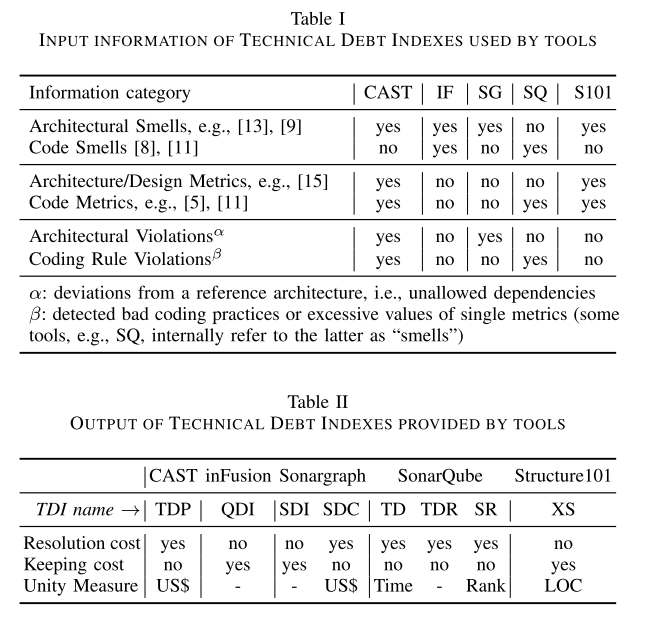
\includegraphics[width=0.5\linewidth]{visualisations/tools-table.png}
	\caption{Summary of tools provided by Fontana et al.}
	\label{fig:tools-tables}
\end{figure}

Unfortunately, there is no standard method of measuring the total technical of a
system. This is due to the complex nature of the metaphor, and one cannot capture
all its complexities into a single tool. Therefore, there is no single best tool
for this purpose, as all take into consideration different sources for metric
computation and it all comes down to the requirements of the team looking to
increase the level of software quality.

%%%%%%%%%%%%%%%%%%%%%%%%%%%%%%%%%%%%%%%%%%%%%%%%%%%%%%%%%%%%%%%%%%%
\subsection{Management}

Although tools provide managers with an approximate measure of the quality of
the code base, there is a danger in associating technical debt with the results
of software quality tools. As mentioned in Section \ref{section:def}, numerous
types of technical debt may have a negative impact on the ROI of the business.
For example, code quality tools cannot predict that the requirements gathering
phase was not completed appropriately or that build debt is affecting
infrastructure costs \cite{Morgenthaler2012}.

Additionally, a study by Martini et al. \cite{Martini2017} showed that the
overall impact of technical debt at the project level is not same as the sum of
all technical debt items. They assessed four projects and interviewed both
project managers and developers on their perspective of the impact, on a scale
from 1 to 10. Although the interviewees had multiple backgrounds and were
consulted on many development factors (reduced development speed, bugs incurred
from technical debt, extra development costs, frequency of issues, users
affected), the results showed that there are other complexities affecting the
project such as social and personal factors.

In an industrial case study \cite{Lim2012}, a developer described technical debt
as follows: ``\textit{Technical debt is a balance between software quality and
business reality}''. Industry practitioners from the same study have
acknowledged that numerous business requirements have forced them to incur debt.
Unfortunately, these requirements and decisions are difficult to foresee due to
constant market deviations, such as the appearance of a new competitor or a new
technology. Therefore, technical debt is difficult to predict. However, many
practitioners recommended that once debt is incurred, it should be made visible
\cite{Lim2012} \cite{Codabux2013} \cite{Morgenthaler2012}, and paid back as
early as possible. Cunningham \cite{Cunningham1993} describes it best:
"\textit{The danger occurs when the debt is not repaid. Every minute spent on
not-quite-right code counts as interest on that debt. Entire engineering
organizations can be brought to a stand-still under the debt load of an
unconsolidated implementation, object-oriented or otherwise.}".

Fortunately, project management methodologies such as Agile and its associated
practices have proved to help reduce and manage technical debt
\cite{Holvitie2014} \cite{Trumler2016}. In particular, Test Driven Development (TDD),
following coding standards, refactoring, continuous integration, collective code
ownership and pair programming have been considered to help tackle technical
debt.

Guo et al. \cite{Guo2011} suggested that technical debt items could be managed
similarly to a financial portfolio perspective by encouraging each item to be
viewed as an investment. Debt items would take on the role of assets, with the
same goals: maximise return and minimise risk. The decision framework could be
based on historical metrics of all debt items to decide which ones to keep and
which ones to pay back. However, the approach is difficult to achieve in
practice due to limitations of the metaphor \cite{Schmid2013}.

Seaman et al. \cite{Seaman2012} proposed four ways to aid in this decision
making:
\begin{itemize}
	\item Cost-Benefit Analysis. The technique uses principal, interest
	      probability (the probability that other work will be more expensive),
	      interest amount and their associated value (high, medium, low) to
	      estimate items that have low principal (are quick to repay) and a
	      possible high impact on future additions and changes.
	\item Analytic Hierarchy Process (AHP). Technical debt items are ranked
	      according to a defined criteria, based on the needs and requirements of the
	      team. A ranked list of items to work on is created through meetings and
	      group decisions.
	\item Portfolio Approach. Guo et al. \cite{Guo2011} have defined an approach
	      for portfolio debt management.
	\item Options. This technique considers that each repayment of debt is an
	      investment in the future. It is similar to a purchase of an option
	      \cite{option-investopedia} that will be called in the future.
\end{itemize}

Power \cite{Power2013} illustrated the impact of technical debt on Agile teams
and methods of management using options, from Cisco System's Agile Office
data-set. He proposed that The items of the portfolio are the slices of time the
team invests in a particular activity. For example, a team may allocate 50\% of
their time to development of new features, 20\% to testing, 15\% to fixing
defects and 5\% resolving technical debt items. An example is displayed in
Figure \ref{fig:td-options}.

\begin{figure}
	\centering
	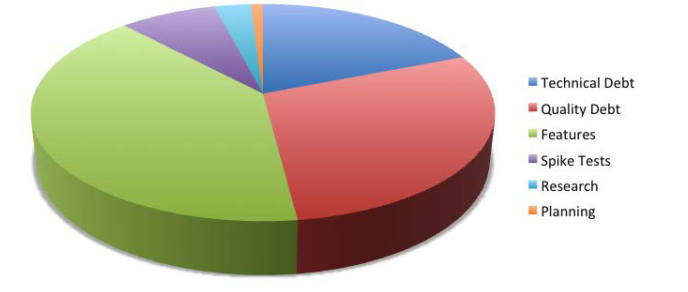
\includegraphics[width=0.5\linewidth]{visualisations/td-options.png}
	\caption{A partitioning example of work effort, provided by Cisco System's Agile Office}
	\label{fig:td-options}
\end{figure}

Similar to previous stages of technical debt, management is no easy feat.
Project managers must balance the work effort, costs with benefits, future
technical impact and return on investment. This can only be possible if
technical debt is visible during software evolution \cite{Lim2012}
\cite{Morgenthaler2012} \cite{Codabux2013}, is continuously tracked and managed
appropriately \cite{Cunningham1993}.

%%%%%%%%%%%%%%%%%%%%%%%%%%%%%%%%%%%%%%%%%%%%%%%%%%%%%%%%%%%%%%%%%%%
\subsection{Conclusion}

Technical debt is a difficult phenomenon to tackle in software engineering.
Development teams face challenges in identifying, tracking, managing and
explaining the concept to non-technical stakeholders. New tools allow the
indentification of code smells, tracking and computing of complex indexes
automatically with focus on quality characteristics of code. There is a danger
in associating technical debt with the result of the static analysis tools as
these tools are not complete and do not take all types of debt into
consideration.

However, code and design debt are the most common type of debt, which developers
and project managers have to deal on a daily basis. The main challenges is
measuring the interest that these types of issues accrue over the lifetime of a
project. It is fair to consider that code and design debt are the primary
sources that directly affect development time and work effort. Therefore,
understanding the interest in terms of work effort may identify future
challenges.

The initial study by Gomes et al. \cite{Gomes2011} provided a good start into
identifying work effort deviation. However, it was only conducted between major
releases of a system and does not provide drill-down data on which features,
code smells and work iterations had the most effect on work effort. This is
essential information for developers and project managers to prioritise
refactoring activities in work iterations, especially in an Agile environment
where responding to change is key \cite{agile-manifesto}.  

%%%%%%%%%%%%%%%%%%%%%%%%%%%%%%%%%%%%%%%%%%%%%%%%%%%%%%%%%%%%%%%%%%%
\section{Proposed Approach}
\label{proposed-work}

This study focuses on finding the relation between technical debt and work
effort. This will yield more information for developers on time management, for
project managers on refactoring investment and for stakeholders on understanding
a technical concept concerning development cost.

The approach for the execution of this study will consist of the following
steps:
\begin{enumerate}
	\item \textit{Identify appropriate data candidates for this study}.\\
	      These are potential software projects that are suitable for study. At
	      best, they should have multiple developers contributing to the
	      project, a medium to large codebase with a variety of historical data
	      and an associated issue tracking software. Ideally, the team would
	      have integrated a continuous code quality tool for tracking code
	      smells throughout software evolution that would help with quick and
	      automatic identification of present and historical code issues.

	      The study would also benefit from a mixture of open-source and
	      commercial software to contrast the differences between the two
	      environments and, possibly, arrive at general conclusions that may
	      apply to both worlds.

	\item \textit{Identify suitable work items from issue tracker}.\\
	      In this step, the purpose is to understand significant events in the
	      evolution of the data candidates. Ideally, events were tracked in the
	      form of tickets with attached detailed information, such as:
	      \begin{itemize}
		      \item \textit{Priority} will give a sense of importance to the work item.
		      Finding development patterns based on this field will be unique.
		      Will developers take more time to design and implement an
		      important work item? Alternatively, are they pressured to deliver
		      and thus introduce more debt in the system?
		      \item \textit{Estimated Work Effort} is one of the most important
		      fields for calculation of extra work effort. This provides the
		      theoretical work time on which to compare the practical work time
		      measured in this experiment. It may be in the form or work hours
		      or story points.
		      \item The opening and closing \textit{timestamps} of a ticket may
		      offer valuable information for measuring the practical work effort
		      in hours, if developers change the status of tickets as
		      development progresses.
	      \end{itemize}

	      Unfortunately this data is not always available. The most important is
	      the estimated work field as without it, the extra work cannot be
	      identified. If this field does not exist in the ticket, the work item
	      will not be included in the study.

	\item \textit{Identify version control checkpoints}.\\
	      Completed work items can be tracked in the version control repository
	      of the project. Identifying checkpoints will aid in understanding the
	      amount of effort put into the work item by the team and how it
	      diverges from the initial estimation.

	      Ideally, the team should have links between revisions of the codebase and
	      the work item in the issue tracker. This would make it easier to find the
	      associated checkpoints.

	\item \textit{Measure the amount of work effort for each work item}.\\
	      The purpose is to understand how many practical changes a work item
	      has induced over its lifetime. This could be done in two ways: at the
	      code and issue tracker levels.

	      At the code level, it is possible to understand the level of work
	      effort involved by aggregating the number of changes a work item has
	      suffered. A changeset consists of the number of lines of code added,
	      deleted and modified. Granularity can be at the pull request, commit,
	      class and method level. Version control systems such as Git provide
	      features for retrieving change sets between revisions.

	      However, identifying work effort from changesets is a challenging
	      task. It is difficult to quantify in working hours since many changes
	      may be generated automatically by modern refactoring tools in the
	      integrated development environment. An alternative solution is to
	      compare the timestamps between the first and the last commit. The
	      temporal difference might provide a practical estimate of work effort
	      to resolve the issue. Unfortunately, this case only works when a
	      developer works on a single issue at a time.

	      At the ticket level, one can understand the amount of work effort
	      realised by a team member. In an ideal case, the team enforces
	      developers to log their time spent designing and implementing a
	      feature. However, that is not always the case. Alternatively, it would
	      be interesting to retrieve the timestamp of ticket events, such as the
	      opening and closing of an issue. Unfortunately, this might not give an
	      approximate time of work since:
	      \begin{itemize}
		      \item The team does not respect the opening and closing of a
		            ticket time according to their development patterns. For
		            example, a developer might start work on an issue before
		            marking it as "In Progress" and thus introduce a margin of
		            error in the estimation process.
		      \item Tickets might remain open for a long period of time, while the
		            feature was implemented in a relatively short time.
		      \item There are differences between commercial and open-source
		            software. For example, developers might work in the
		            timeframe of 9 AM to 6 PM in commercial environment while in
		            open-source they are free to work at any time of the day.
		            For example, in an extreme case, a developer marks a ticket
		            as ``In Progress'' before the end of the working day, and
		            resume working the following morning. In this case, our
		            estimation of approximately 15 hours of development time for
		            this work item would be incorrect.
	      \end{itemize}

	      For this study, the code level technique will be implemented. The work
	      effort from issue tracking will be implemented in a parallel study.
	      However, it would be interesting to gather results from both methods
	      and see how they correlate. Additionally, the two result sets may
	      complement one another and provide an overall effort metric. However,
	      as discussed, there are many complexities and cases that will need to
	      be managed to get the real estimate.

	\item \textit{Measure technical debt items}.\\
	      The scope of this step is to identify code violations within
	      changesets. For each work item implemented there will be a set of
	      associated modules, classes and methods affected.

	      Historical code smells can be identified and tracked within the
	      evolution of changesets using a continuous code quality tool. If
	      enough data is available, then patterns surrounding feature
	      implementation and bug fixing can be identified.

	      Ideally, the team would have the code quality tool integrated into
	      their continuous integration environment. If so, then historical code
	      smell data could be leveraged by retrieving it through an API.
	      However, that is not always the case. Therefore, a code quality tool
	      must be used to analyse the version control checkpoints identified and
	      find code smells that may have an impact on change sets of a feature.

	\item \textit{Analysis and discussion of results}.\\
	      The three data sources can be linked together once all steps are
	      fulfilled. Extra work can be correlated to issue tracking information
	      and code quality at the time of development. Technical debt could be
	      classified by the type, priority, code smells and assignee.
\end{enumerate}

Unfortunately, the proposed work is not as straightforward. There are many
complexities of the work environment which cannot be considered from the three
data sources. Therefore, we will make some assumptions:
\begin{itemize}
	\item The team uses Git for version control and follows the pull request model
	      for implementing changes.
	\item Only one developer is assigned to an issue.
	\item A developer works on maximum one issue at a time.
	\item The team uses an issue tracker consistently. Developers change the
	      status of the ticket according to their current development progress.
	      For example, if a team member got started on a work item, she would
	      set the ticket status to ``In Progress''. Respectively, she would mark
	      the ticket as ``Closed'' if development ceased, her changes were
	      reviewed and integrated into the main branch.
	\item The team estimates the theoretical amount of work necessary to
	      implement a feature or fix a bug. This measure is attached to each
	      work item selected.
	\item Development time is between 9 AM to 6 PM UTC. Only work items with
	      opening and closing status between these two values are taken into
	      consideration. For example, if a developer starts work on a feature on
	      Monday 5 PM and finishes it by Tuesday 1 PM, then development time
	      will be considered to be 4 hours (1 hour Monday, 3 hours Tuesday).
	      This assumption will simplify the calculation of reasonable work hours
	      for work items.
\end{itemize}

These assumptions will reduce the amount of real-world complexity in the
experiment and allow for simple validation of the results. Additionally, the
complexities may be explored in future studies.

\subsection{Limitations}

As discussed in Section \ref{section:def} there are multiple types of debt
affecting the software environment which cannot be modelled in this study.
Additionally, with the introduction of assumptions to limit the complexity of
the study, there are many threats to the validity of the results.

\begin{itemize}
	\item Data candidates may not have sufficient information related to the
	      estimation of work effort. We believe this statement is especially
	      true for open-source software, with an international team and
	      contributions from many other developers. Although care will be taken
	      in the selection process, there is no assurance that this data will
	      exist. However, if commercial projects do have estimation fields, it
	      would be interesting to correlate the amount of practical work done
	      between the two worlds for similar tickets.
	\item Work effort measurement is a difficult challenge and was deemed
	      unmeasurable by Martin Fowler \cite{CannotMeasureProductivity}. We
	      consider work effort measurement as the time taken to deliver the
	      requirements, assuming that all requirements of a system in
	      development brings an associated business value. Restricting
	      development time to an interval and discarding multi-developer work
	      items may reduce the data set considerably.
	\item Code quality tools may not detect potential technical debt items. For
	      example, architectural debt is an essential factor in assessing extra
	      work but this type of debt which was not included due to its
	      complexity.
	\item The assumptions made in the previous section may not reflect the real
	      work environment. Developers may be working overtime if, for example, under
	      the pressure of a release schedule.
	\item There are many types and complexities of technical debt which were not
	      included. Requirements, architectural, build, infrastructure and test
	      have an influence on the amount of effort for finalising a feature.
\end{itemize}

Although there are risks associated with measurements, care will be taken to
consider all possibilities when validating calculation of measurements. This is
especially true in the case of quantifying work effort.

%%%%%%%%%%%%%%%%%%%%%%%%%%%%%%%%%%%%%%%%%%%%%%%%%%%%%%%%%%%%%%%%%%%
\section{Work Plan}
\label{work-plan}

Considering the proposed work in Section \ref{proposed-work}, work packages can
be easily created by identifying activities. These activities could be placed in
time slots, spanning 11 weeks worth of experimental work from January 2018 until
April 2018. The work packages and activities are as follows:

\begin{enumerate}
	\item \textit{Gathering data}.\\
	Activities included:
	\begin{itemize}
		\item Identify suitable commercial and open-source software projects.
		\item Familiariase with development environment of enterprise software
		and possible limitations of the work involved.
		\item Select appropriate code quality tools that support the programming
		language of the software.
		\item Identify important work items relevant for the study, including
		items such as features, bugs, refactoring activites and enhacements.
	\end{itemize}

	Estimated work time: 3 weeks.\\
	
	\item \textit{Development of automated tools}.\\
	Activities included:
	\begin{itemize}
		\item Design and develop a tool for retrieving ticket information from
		the project issue tracker.
		\item Design and develop a tool for changing between revisions of the
		source code, for measuring effort by changesets and storing timestamps
		between revisions.
	\end{itemize}

	Estimated work time: 3 weeks.\\

	\item \textit{Measuring technical debt}.\\
	Activities included:
	\begin{itemize}
		\item Use selected code quality tool on work revisions to identify code
		smells within changesets.
		\item Integrate the code quality tool features with the previous tool
		for measuring revision effort.
	\end{itemize}

	Estimated work time: 2 weeks.\\

	\item \textit{Data Verification and Analysis}.\\
	Activities included:
	\begin{itemize}
		\item Analyse data integrity for inconsistencies and remove outliers.
		\item Statistically test the correlation between work effort and technical debt.
	\end{itemize}

	Estimated work time: 3 weeks.\\

	\item \textit{Presentation of results and report writing}.
	Activities included:
\begin{itemize}
	\item Present the results to project supervisor and enterprise
	representatives.
	\item Write the final report.
\end{itemize}
	Estimated work time: 3 weeks.\\

\end{enumerate}

%%%%%%%%%%%%%%%%%%%%%%%%%%%%%%%%%%%%%%%%%%%%%%%%%%%%%%%%%%%%%%%%%%%
\section{Conclusion}

To conclude, technical debt is a phenomenon difficult to measure accurately and
assess potential development and business costs. Therefore, understanding it
from the perspective of developers is vital as they are first-hand involved in
the implementation of new features. Any extra work spent as a result of previous
incurred debt increases business costs. If too much debt accrues over the
lifetime of a project, the entire project may be brought to a stand-still.

As a result, this study will try to understand technical debt from a development
work effort perspective. It will, possibly, shed light on the types of features
that take a lot of man-hours to complete in correlation with the level of
technical debt at the present time of the implementation. 

Through measurement and analysis of these two metrics and their relationship,
developers may discover bottlenecks in productivity, managers may allocate
appropriate resources for refactoring activities and business stakeholders may
become more aware of development concerns. Additionally, it will be interesting
to find the discrepancy between open-source and proprietary software projects.

To the best of my knowledge, this type of study had not been conducted before
from the perspective of work effort at the feature level granularity and may
provide valuable insights into the development patterns of software engineering.

%%%%%%%%%%%%%%%%%%%%%%%%%%%%%%%%%%%%%%%%%%%%%%%%%%%%%%%%%%%%%%%%%%%
% it is fine to change the bibliography style if you want
\pagebreak
\bibliographystyle{plain}
\bibliography{mprop}
\end{document}
